%\documentclass{article}
%\usepackage{paralist} 
%\usepackage{graphicx}
%\begin{document}


\section{Security Lab Generator}
Security Lab Generator (SLG) is a research project that is aimed to configure, deploy, monitor and analyze the network environments regarding security issues. The report contains an overview of the project, an overview of third-party components used in the SLG, ideas about use cases and proposals how SLG could be used for automation of the testbed creation for research in the IT security area.

\subsection{Overview}

In this section we use follow definitions:
\begin{compactitem}
\item Scenario - a formal description of the computer network. 
\item Attack graph - another view of the scenario that describes possible attacks against the certain network environment regarding on the location of the attacker and the hacking targets.   
\item Experiment - a virtualized network with all needed hosts and software applications according to a specific scenario.
\item Provision server - a server for hosting the experiment. In the current case, the provision server is VirtualBox.
\end{compactitem}

\begin{figure}[ht!]
\centering
%[width=90mm]
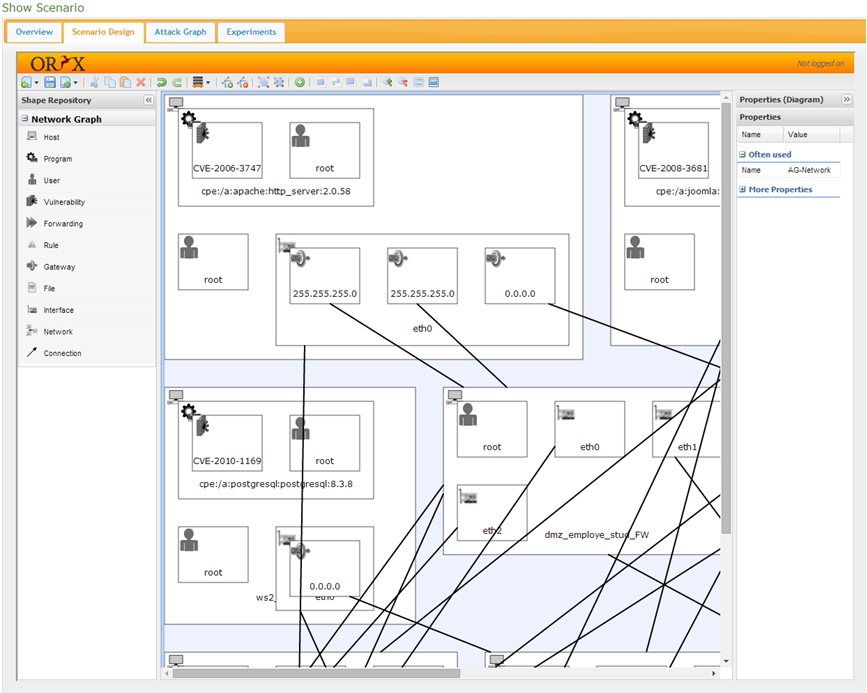
\includegraphics[width=\textwidth]{slg.png}
\caption{SLG}
\label{overflow}
\end{figure} 

The SLG project uses additional projects: Oryx [2] for prototyping the network environment, MulVAL [3] for analyzing the network environment by creating attack graphs and VirtualBox for running virtual machines. SLG is written on the java programming language with the grails framework and uses the Tomcat server and the MySql database. Oryx uses additional components such as the PostgreSQL database and the PLPython library[4]. MulVAL is a logic-based enterprise network security analyzer and it is used for creating an attack graph based on the prototyped scenario, which can be represented as an image with relations, as well as a xml file. Also MulVAL requires additional modules: XSB [5] - a logic programming and deductive database system and GraphViz [6] - a graph visualization software. 

The important parts of SLG are image pool and program pool. The image pool is the container of prepared virgin images of operations systems, which can be used for deploying virtual machines. The program pool is the container of software programs, which can be used for being installed on virtual machines. Any new image and the program can be added to the pools.

SLG uses the Oryx application for prototyping the network. You can see the user interface of SLG with the open Oryx editor on Figure 4. The result of prototyping can be exported as json or xml format, which is describing the network scenario. The SLG XML can be converted to the input xml suitable for being used in MulVAL. 

After prototyping the network, specifying each nodes and viewing the attack graph you can prepare and execute the experiment. The process of preparing the experiment includes the creation of virtual machines with operating systems, the installation of software applications and the configuration of the network. After the experiment is prepared, all resources will be installed and configured on VirtualBox. Also SLG provides capability to connect to each virtual machine from the web interface. 


SLG can be used in multiple use cases, but the main goal is to provide the platform for teaching network security issues and the creation testbeds for research in the area of network security and security analytics. 
As a platform for teaching, SLG can be used for Capture the Flag (CTF) seminars. The idea of the seminar is that the tutor deploys a potentially vulnerable network with vulnerable applications. Students, in turn, are trying to gain access to the network and virtual machines using found vulnerabilities to find flags, which are some labels or codes. SLG should provide capability not only to deploy the network environment, but also to monitor user activities, find out compromised machines, make a report on ways of hacking the system. They will be research challenges in the scope of the topic.
  
  
%In this section we just learned Security Lab Generator. On the next section we will introduce the OpenStack technology and the proposal of migrating SLG on the cloud.
 %"4.4 Security Lab Generator based on OpenStack". 


 

%The current state of the project does not allow to use it for real seminar. SLG requires %implementation of some necessary features. 



\subsection{OpenStack at HPI}
OpenStack is a free and open-source infrastructure as a service that provides capability to run any complex network environments [7]. To learn OpenStack and learn how OpenStack could be used as a basement for SLG, a testing infrastructure was deployed on the HPI server with installed VMware ESXi. The deployed infrastructure includes several services: Identity (Keystone), Compute (Nova), Image service (Glance), Networking (Neutron), Block Storage (Cinder), Object Storage (Swift), Dashboard (Horizon), Orchestration (Heat), Telemetry (Ceilometer). In the brackets are code names of services. 
\begin{figure}[ht!]
\centering
%[width=90mm]
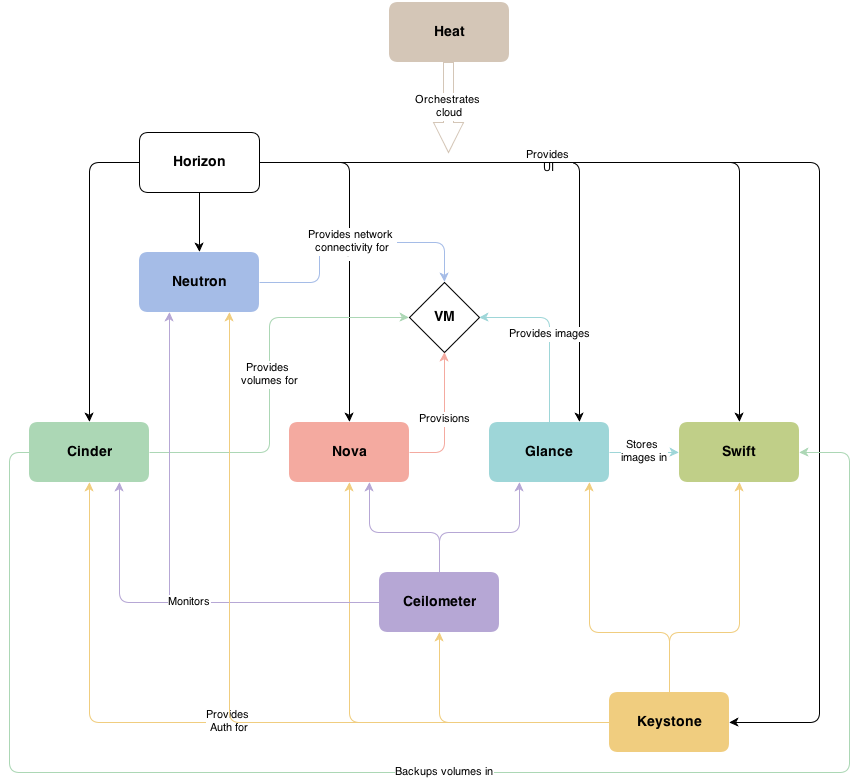
\includegraphics[width=\textwidth]{openstack_conceptual_architecture.png}
\caption{OpenStack conceptual architecture}
\label{overflow}
\end{figure}
The Figure 5 shows relations between services and on the Figure 6 you can see all VMs that were used for deploying OpenStack services. Theoretical, all services could be deployed on one VM and even there is a tool for that called DevStack\footnote{DevStack. http://devstack.org.}. But it is not option for learning or providing the basement for SLG. Our test deployment uses the Icehouse version of OpenStack, Ubuntu operation system and three networks: external, management and instance tunnels. The external network is a network segment typically used for instance Internet access. The management network is a network segment used for administration, not accessible to the public Internet. The instance tunnels network is a network segment used for instance traffic tunnels between compute nodes and the network node.  

\begin{figure}[ht!]
\centering
%[width=90mm]
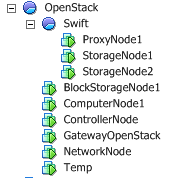
\includegraphics{openstack_tree.png}
\caption{OpenStack nodes}
\label{overflow}
\end{figure}


%\begin{figure}[ht!]
%\centering
%[width=90mm]
%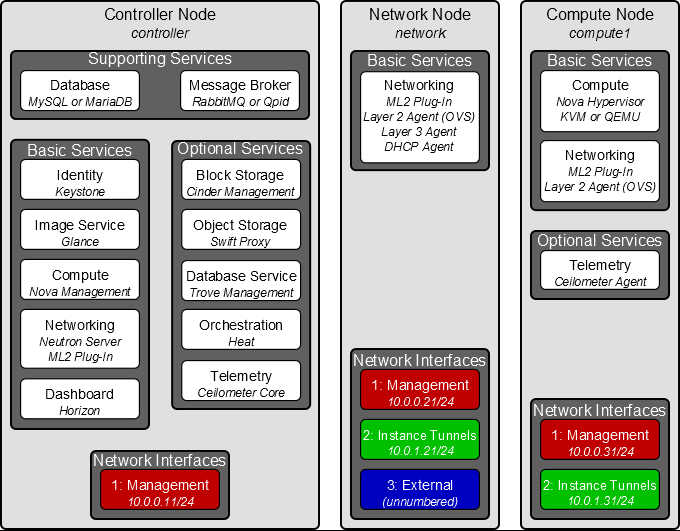
\includegraphics[width=\textwidth]{openstack_architecture.png}
%\caption{OpenStack architecture}
%\label{overflow}
%\end{figure}

The sections just cover basic information about OpenStack. To learn more, please visit official web site [7]. On the official web site you can find all needed information about OpenStack, each service, the installation documentation and other relevant information. 


\subsection{Security Lab Generator based on OpenStack}
The idea of Security Lab based on OpenStack (CloudSLG) is the migration of the current SLG project on the cloud. Firstly, it will allow to use the wide functionality of the IaaS in the interests of SLG. It means that we will not need care about how to create, set up the network, how to connect to running instances. Secondly, it will push forward our goal to automate the creation of testbeds for research in the area of network security and security analytics. Thirdly, it will allow to concentrate on solving more research questions such as analyzing user activities, finding user's attack graphs, reporting analytic statistics. To migrate SLG on the cloud and automate the testbed creation, some challenges must be solved. The first challenge is how to convert the SLG XML into the CloudFormation\footnote{CloudFormation. http://aws.amazon.com/cloudformation} language which is used in OpenStack as well as in Amazon Web Service for running a network stack. The second challenge is how to provide the automation of creating specific images with vulnerable software applications.



%\end{document} 